\section{Theoretical Background}

\subsection{Related Works}

The domain of Image Classification has experienced tremendous development over the last few decades, propelled by the increase in computational capabilities, large amounts of available data, and the development of sophisticated algorithms. This section provides an overview of the major advancements in the field of Image Classification, especially for its applications in industrial environments, such as electronics manufacturing. We will also explore the increasing significance of anomaly detection, emphasizing the transition from conventional supervised learning approaches to modern unsupervised learning methods.

\subsubsection{Evolution of Image Classification Techniques}

Image Classification is a critical task in the field of \gls{cv}, with numerous applications ranging from medical diagnostics to autonomous driving. Early image classification algorithms mainly relied on manual feature extraction, which involves domain experts designing these features, which could be used to differentiate between classes of images. These features were subsequently inputted into traditional machine learning algorithms like \glspl{svm} or \gls{k-nn} for classification \cite{LeCun2015}. Nevertheless, these techniques were limited by their dependence on handcrafted features, which could not effectively reflect intricate changes observed in real-world scenarios.

Subsequently, the introduction of \glspl{cnn} was a significant milestone in this field. They have introduced the concept of feature learning, whereby the network learns to extract relevant features from the raw image data by using numerous layers of convolutional filters \cite{NIPS2012_c399862d}. This groundbreaking study in \cite{NIPS2012_c399862d} on AlexNet architecture delivered exceptional results on the ImageNet dataset for image classification. This success triggered various research into network architectures that are deeper and more complex, such as VGGNet \cite{simonyan2015deepconvolutionalnetworkslargescale}, GoogLeNet \cite{7298594}, and ResNet \cite{he2016deep}.

Among these, the work on the introduction of ResNet by \cite{he2016deep} was highly significant as it addressed the issues of vanishing gradients that tormented earlier deep networks \cite{simonyan2015deepconvolutionalnetworkslargescale} \cite{7298594}. ResNet made it possible to train much deeper networks by incorporating residual connections, resulting in substantial improvement in accuracy over various image classification benchmarks. Thus \glspl{cnn} were firmly established as the leading approach for tasks like image classification.

\subsubsection{Applications of Image Classification in Industrial Settings}

In the industrial sector, special attention is given to image classification applications in quality control processes, particularly in the context of automated visual inspection. Traditionally, the visual inspection process was carried out manually, where we had to rely on the experience of quality inspectors to ensure product quality. As a result of the varying levels of expertise among inspectors and the limitations of human abilities, this approach exhibits low efficiency, low accuracy, and inadequate real-time performance on a large-scale manufacturing process \cite{Gong_2020}.

With the rise of \gls{dl}, automated visual inspection systems are developed using \glspl{cnn} for defect detection in real-time. One of the most notable models in industrial applications is \gls{yolo} which is used for real-time object detection and has gained popularity in tasks requiring rapid image processing. The design of \gls{yolo} enables it to perform object detection in a single iteration over the network, rendering it highly efficient in cases where speed is critical. For example, during the PCB manufacturing process, \gls{yolo} can rapidly identify solder joints that do not meet quality standards. This offers a significant decrease in inspection times as compared to traditional manual techniques \cite{redmon2016you}.

Although \gls{cnn}-based models such as \gls{yolo} have demonstrated their effectiveness in most industrial applications, they do have certain limitations. One of the major obstacle is the requirement for a large labeled dataset to properly train such models. In many industrial applications, such as PCB inspection, defects are rare, and gathering labeled instances in large enough quantities for training purposes may become prohibitively expensive. In such instances, the labeling process is typically very labor- and knowledge-intensive, resulting in high costs and time consumption\cite{FINK2020103678}.

\subsubsection{Anomaly Detection in Electronics Manufacturing}

Due to the lack of labeled data, supervised learning methods are not feasible in certain scenarios. As a result, there has been a growing interest in exploring unsupervised learning methods for anomaly detection. Anomaly detection is the process of identifying patterns in data that deviate from expected behavior. This makes it an suitable solution in industrial applications for identifying defects where normal instances are well represented but anomalies are rare and diverse \cite{10.1145/1541880.1541882}.

In electronics manufacturing, anomaly detection plays an important role for tasks like solder joint inspection. Traditional techniques are based on models like probabilistic and distance-based. These techniques, are effective when dealing with simpler anomaly patterns but often faces difficulties when dealing with complex and high-dimensional data, as explained by \cite{PIMENTEL2014215}. This article points to the limitation of these methods because they reply on predefined thresholds and basic data assumptions, that fails to generalize on wide variety of anomalies.

Further expanding on this foundation, recent advancements in \gls{dl} introduced more sophisticated methods, particularly by employing autoencoders\cite{bank2021autoencoders}. Neural networks, namely \glspl{vae}\cite{Kingma_2019}, provides substantial improvements in presenting complex data distributions. These autoencoders learns compression and reconstruction of inputs through training on normal operational data, thereby building a model of 'normality' that allows it to find those anomalous instances with higher reconstruction errors indicating a deviation from the normal\cite{bank2021autoencoders}. This approach improves the detection of complex patterns of defects to help maintain the integrity of products produced in the manufacturing processes. Other variants of autoencoders, such \gls{vae}, deep autoencoders, has been investigated for anomaly detection and has shown promising results \cite{Kingma_2019}.

Another increasingly popular method is the \glspl{gan}\cite{goodfellow2014generativeadversarialnetworks} for anomaly detection. \glspl{gan} is consisting of two networks, namely a generator and a discriminator, both are trained simultaneously. The generator tries to produce data that is indistinguishable from the real one, while a discriminator strives to differentiate between real and generated data. In the context of anomaly detection, the generator is trained to generate normal instances, while the discriminator learns to identify any deviations from this normal distribution as anomalies \cite{schlegl2017unsupervisedanomalydetectiongenerative}.

%\subsubsection{Gaps in Current Research}

%Although significant advancements have been made in image classification and anomaly detectionusing both supervised and unsupervised learning methods, there are still certain gaps in the current research. The most obvious obstacle is the effective integration of the two approaches that maximizes the advantages of each other. Although supervised models, such as \gls{yolo}\cite{redmon2016you}, succeed well with abundant labeled data, they struggle in applications where labels are limited or where anomalies have not been well-defined. While unsupervised models entail more flexibility and typically require less labeled data, many are incapable of pulling off the same level of precision achieved with supervision when it comes to fine-grained classification tasks \cite{9347460}.




%In recent years, the exponential growth in deep learning research has revolutionized the field of Computer Vision. Much of this change has been led by Convolutional Neural Networks (CNNs), making highly accurate image recognition tasks possible[1]. Since then, ResNet and EfficientNet have further moved this needle by resolving issues like vanishing gradients and model scaling optimization[2][3]. Moreover, Vision Transformers (ViTs) have provided a new perspective in image classification by using transformer architectures primarily tailored for natural language processing[4]. These innovations have extended the scope of various areas in which deep learning applications can be applied in different industries, enhancing the ability to analyze and interpret complex visual data.

%The application of image classification techniques in the electronics manufacturing industry has shown significant promise. Automated visual inspection systems utilizing CNNs can effectively identify and classify defects in various manufacturing processes, reducing the reliance on manual inspection and minimizing human error. For example, deep learning models have been successfully applied to detect defects in automotive parts, textile production, and food processing, demonstrating their versatility and effectiveness [5]. Moreover, the integration of these techniques has streamlined quality control processes, enabling faster and more accurate identification of defects, which is crucial for maintaining high standards of product quality and efficiency in production lines [6].

%Advances in anomaly detection, particularly through unsupervised learning, have also played a critical role in the manufacturing sector. Traditional methods often rely on labeled datasets, which can be time-consuming and costly to generate. Unsupervised anomaly detection techniques, such as autoencoders, variational autoencoders (VAEs), and generative adversarial networks (GANs), have alleviated this dependency by identifying deviations from normal patterns without the need for extensive labeling [7]. These methods have been applied to detect anomalies in a wide range of manufacturing contexts, from monitoring machinery health to ensuring the integrity of assembled products. By leveraging the inherent patterns in the data, unsupervised learning approaches have enabled more scalable and adaptable solutions for anomaly detection [8][9].

%The continuous evolution of these technologies underscores the transformative impact of deep learning on the manufacturing industry. By integrating advanced image classification and anomaly detection techniques, manufacturers can achieve more efficient and accurate inspection processes, ultimately leading to improved product quality and operational efficiency. This ongoing research and development highlight the potential for even greater advancements in the future, as deep learning models become more sophisticated and capable of addressing increasingly complex manufacturing challenges [10].

%References

%[1] Krizhevsky, Alex, Ilya Sutskever, and Geoffrey E. Hinton. "Imagenet classification with deep convolutional neural networks." Advances in neural information processing systems 25 (2012).
%[2] He, Kaiming, et al. "Deep residual learning for image recognition." Proceedings of the IEEE conference on computer vision and pattern recognition. 2016.
%[3] Tan, Mingxing, and Quoc V. Le. "EfficientNet: Rethinking model scaling for convolutional neural networks." International Conference on Machine Learning. PMLR, 2019.
%[4] Dosovitskiy, Alexey, et al. "An image is worth 16x16 words: Transformers for image recognition at scale." arXiv preprint arXiv:2010.11929 (2020).
%[5] Bhandarkar, Suchendra M., et al. "Deep learning based quality inspection in manufacturing." Procedia Manufacturing 26 (2018): 998-1006.
%[6] Zhang, Xiaolei, et al. "Deep learning-based quality inspection for manufacturing." IEEE Access 7 (2019): 61232-61245.
%[7] An, Jinwon, and Sungzoon Cho. "Variational autoencoder based anomaly detection using reconstruction probability." Special Lecture on IE 2.1 (2015).
%[8] Ruff, Lukas, et al. "Deep One-Class Classification." International Conference on Machine Learning. PMLR, 2018.
%[9] Kiran, B Ravi, Dilip Thomas, and Ranjith Parakkal. "An overview of deep learning based methods for unsupervised and semi-supervised anomaly detection in videos." Journal of Imaging 4.2 (2018): 36.
%[10] Bergmann, Paul, et al. "Uninformed students: Student-teacher anomaly detection with discriminative latent embeddings." Proceedings of the IEEE/CVF Conference on Computer Vision and Pattern Recognition. 2020.

%\subsection{Machine Learning}

%Machine Learning is a subdomain of Artificial Intelligence that encompasses various techniques able to automatically discover patterns in data and use those patterns to predict future data[1].

\subsection{Supervised Image Processing}

\subsubsection{Artificial Neural Networks (ANNs)}

\gls{ann} are computational processing systems that are inspired by how biological nervous systems such as the human brain functions. \gls{ann} mainly consists of numerous interconnected computational nodes, known as neurons, which are intertwined in a distributed manner to collectively learn from te input and optimize the final output \cite{oshea2015introductionconvolutionalneuralnetworks}.

\begin{figure}[ht!]
    \centering
    \includegraphics[width=1\linewidth]{Images/ann_architecture.pdf}
    \caption{\gls{ann} is a three-layer \gls{fnn} consisting of an input layer, a hidden layer, and an output layer \cite{oshea2015introductionconvolutionalneuralnetworks}.}
    \label{fig:ann architecture}
\end{figure}

The figure \ref{fig:ann architecture} shows the basic structure of a \gls{ann}. Input data will be loaded in the form of multidimensional vector into the input layer, then it will be distributed into the hidden layer. Then hidden layers will make decisions based on previous layer and evaluate how a stochastic change improves the final output, this process is know as learning. When multiple hidden layers are stacked next each other it is known as \gls{dl} \cite{oshea2015introductionconvolutionalneuralnetworks}.

\subsubsection{Convolutional Neural Networks (CNNs)}

\glspl{cnn}\cite{726791} is an extended version of \gls{ann} which is primarily used for feature extraction from a grid-like matrix dataset \cite{GeeksforGeeks2024}. \glspl{cnn} is similar to traditional \gls{ann} in terms of that they consists of neurons that self-optimize through learning. Each neuron will receive input and perform operations like scalar product followed by a non-linear function, which is the basis of many \gls{ann}. The only significant difference between \glspl{cnn} and traditional \gls{ann} is that \glspl{cnn} are mainly used on images in the field of pattern recognition. This enables the encoding of image-specific features into the architecture, making it more suitable for image-focused tasks while also reducing the parameters required for model configuration \cite{oshea2015introductionconvolutionalneuralnetworks}.

The term \glspl{cnn} indicates that the network uses a mathematical operation called \textbf{convolution}. \glspl{cnn} are neural networks that in the place of general matrix multiplication uses convolution in at least one of the layers \cite{Goodfellow-et-al-2016}.

\paragraph*{\gls{cnn} Architecture :}

Basic \gls{cnn} architecture consists of three types of layers, they are \textbf{convolutional layers}, \textbf{pooling layers}, and \textbf{fully connected layers}. When these layers are stacked together, then a \gls{cnn} architecture is formed. Figure \ref{fig:cnn architecture} shows \gls{cnn} architecture for MNIST\cite{6296535} classification.


\begin{figure}[ht!]
    \centering
    \includegraphics[width=1.1\linewidth]{Rohit_Master_Thesis//Images/cnn_architecture.pdf}
    \caption{A common \gls{cnn} architecture \cite{oshea2015introductionconvolutionalneuralnetworks}}
    \label{fig:cnn architecture}
\end{figure}

The functionality of \gls{cnn} architecture shown above can be broken down basically into four key areas.

1. Similar to other types of \gls{ann}, the input layer holds the images pixel values \cite{oshea2015introductionconvolutionalneuralnetworks}.

2. Convolutional layer will determine the output of neurons that are linked to local regions of input by calculating the scalar product of their weights and the corresponding input volume region. The \gls{relu} aims to apply an 'elementwise' activation function like sigmoid to the output generated by the preceding's layer's activation \cite{oshea2015introductionconvolutionalneuralnetworks}.

3. The pooling layer will perform downsampling along the spatial dimensions of the input, this further reduces the number of parameters in the activation \cite{oshea2015introductionconvolutionalneuralnetworks}.

4. The fully connected layers will then perform the same functions as that in a standard \gls{ann}, aiming to produce class scores from the activations, for classification purposes. To improve performance, it's also recommended to use \gls{relu} between these layers \cite{oshea2015introductionconvolutionalneuralnetworks}. 

By using this simple transformation technique, \glspl{cnn} can transform the original input layer by layer, by using convolutional and downsampling techniques producing class scores for classification and regression purposes \cite{oshea2015introductionconvolutionalneuralnetworks}. Lets look at the main components of the \gls{cnn} architecture in detail.

\paragraph*{Convolutional Layer :}

Convolutional layer plays important role in the \glspl{cnn} functionality. The layers parameters concentrate on the use of learnable \textbf{kernels}. These kernels are the set of learnable parameters.

These kernels are usually small in spatial dimensions, however spreads entirely along the depth of the input. Upon the data entering a convolutional layer, it convolves each filter across the spatial dimensions of the input to generate a 2D activation map as shown in figure \ref{fig:convolutional layer} \cite{oshea2015introductionconvolutionalneuralnetworks}.

%\begin{figure}
%    \centering
%    \includegraphics[width=1.1\linewidth]{Rohit_Master_Thesis//Images/conv_layer.pdf}
%    \caption{A visual representation of a covolutional layer. The centre element of the kernel is positioned over the input vector, from which then a weighted sum of itself and any nearby pixels is calculated and replaced \cite{oshea2015introductionconvolutionalneuralnetworks}.}
%    \label{fig:convolutional layer}
%\end{figure}

\begin{figure}[ht!]
    \centering
    \includegraphics[width=1\linewidth]{Rohit_Master_Thesis//Images/conv_layer_v2.png}
    \caption{The convolution operation involves the sliding of a convolution kernel(filter) over the input vector, where the kernel is multiplied by the pixel value at the corresponding positions of the input, and summing them to produce a feature map \cite{Zhao2024}.}
    \label{fig:convolutional layer}
\end{figure}

As the kernel glides through the input, it calculates the scalar product for each value in that kernel. Through this the network will learn kernels that activates upon they detect a specific feature at a given spatial position of the input. These are commonly referred to as activations. Each kernel will have a corresponding activation map, which will be stacked along the depth dimension to form complete output volume from the convolutional layer \cite{oshea2015introductionconvolutionalneuralnetworks}.

To mitigate the problem of \gls{ann} where the models gets too big to train effectively due to the full-connected nature of standard \gls{ann} neurons, each neuron in a convolutional layer is connected only to a small region of the input, known as \textbf{receptive field}. The connectivity depth is almost always equal to the input depth \cite{oshea2015introductionconvolutionalneuralnetworks}. To understand this, lets consider an example, if the network receives an input image measuring $64\times64\times3$(representing an RGB image), with the receptive field being of the size $6\times6$, each neuron will have a total of 108 weights with in the convolutional layer($6\times6\times3$, with 3 representing the amount of connectivity across the depth of the volume). Whereas a standard neuron in other forms of \gls{ann} would have $12,288$ weights each \cite{oshea2015introductionconvolutionalneuralnetworks}.

By optimizing its output convolutional layers can also significantly reduce the complexity of the model. These are optimized by three hyperparameters: depth, stride, and setting zero-padding.

The \textbf{depth} of the output volume can be set manually using the number of neurons within the convolutional layer corresponding to the same region in the input. Although reducing this hyperparameter can significantly reduce the total number of neurons of the network, it can also significantly reduce the model's pattern recognition capabilities \cite{oshea2015introductionconvolutionalneuralnetworks}.


\textbf{Stride} is the number of rows and columns that the receptive field will move across the input's spatial dimension \cite{Zhao2024}. For example, with stride set to 1, then the significantly overlapping receptive field will produce very large activations, while a larger value of stride will reduce overlapping and produce an output of lower spatial dimensions \cite{oshea2015introductionconvolutionalneuralnetworks}.

\textbf{Zero-Padding} is a simple process of padding the border of the input with zeros, it's an effective way to enhance control of the dimentionality of the output volumes \cite{oshea2015introductionconvolutionalneuralnetworks}.

We can calculate the spatial dimensionality of convolutional layers output by using the following formula: 

\[
    \frac{(V - R) + 2Z}{S + 1}
\]

Here the V denotes the input volume size(height$\times$width$\times$depth), R denotes the receptive field size, Z denotes the zero-padding set, and S denotes the stride. If the result from the above formula is not a whole integer then the stride has been set incorrectly, and the neurons wont be able to fit across the given input \cite{oshea2015introductionconvolutionalneuralnetworks}.

Despite these optimizations, models can still be huge while using high dimensionality input like images. To further reduce the number of parameters significantly within the convolutional layer \textbf{parameter sharing} is used. It works on the assumption that if a feature from one spatial region is useful for computation, then its likely to be useful in another region as well \cite{oshea2015introductionconvolutionalneuralnetworks}.

\paragraph*{Pooling layer :}

The pooling layers reduces the dimensionality of the feature representation, thus reducing the number of parameters and computational complexity of the model. Pooling layer operates on each activation map in the input, and reduces its dimensionality using the 'Max' function. Max-pooling layers is one of the most common types of pooling used in \glspl{cnn}. It selects the maximum activity value of all neurons for the representation for the particular region and extract the most essential feature from the input feature map \cite{Zhao2024}. A $2\times2$ kernels is applied with a stride of 2 across the spatial dimensions of the input reduces the activation map by $75\%$ of the original size, while preserving the depth volume of the feature map \cite{oshea2015introductionconvolutionalneuralnetworks}. 

Average pooling computes the arithmetic mean of all the elements within the region, resulting in the mean value of the local response from the extracted feature mapping \cite{Zhao2024}. The figure \ref{fig:max pooling} shows max pooling operation where the maximum value is used, and figure \ref{fig:average pooling} shows the average pooling operation, which performs the average operation to get the value.

\begin{figure}[H]
    \centering
    \includegraphics[width=1\linewidth]{Rohit_Master_Thesis//Images/max_pooling.png}
    \caption{Max pooling \cite{Zhao2024}}
    \label{fig:max pooling}
\end{figure}

\begin{figure}[H]
    \centering
    \includegraphics[width=1\linewidth]{Rohit_Master_Thesis//Images/average_pooling.png}
    \caption{Average pooling \cite{Zhao2024}}
    \label{fig:average pooling}
\end{figure}

\paragraph*{Fully-Connected Layer :}

The fully-connected layer contains neurons which are directly connected to the neurons in the two neighboring layers, with no connections to any neurons within itself. It is similar to the way neurons are arranged in traditional \gls{ann} as can be seen in the figure \ref{fig:ann architecture} \cite{oshea2015introductionconvolutionalneuralnetworks}.

\paragraph*{Activation Function :}

Activation functions plays a crucial role in neural networks, strengthening the network's representational and learning capabilities, by learning the abstract features through nonlinear transformation \cite{dubey2022activationfunctionsdeeplearning}. With the introduction of the activation functions, the neural network can approximate any nonlinear function, making it applicable to a wide range of nonlinear models \cite{Zhao2024}. Some of the activation functions common properties are:

1. It should add the nonlinear curvature in the optimization landscape to enhance training convergence of the network;

2. It shouldn't significantly increase the computational complexity of the model;

3. During training it shouldn't hamper the gradient flow;

4. It should preserve the data distribution and facilitate better network training \cite{dubey2022activationfunctionsdeeplearning}.

Here we will look at the most common and widely used activation functions, including Sigmoid, Tanh, Softmax, \gls{relu}, and Leaky \gls{relu}.

\textbf{1. Sigmoid Activation Function :}

The Sigmoid function, or the logistic function, ranges from 0 to 1. As can be seen from the figure \ref{fig:sigmoid tanh function curve}, sigmoid can be used to normalize the output, as well as probability-based predictions \cite{Zhao2024}. The following is the sigmoid functions mathematical formula :

\[ 
    f(x) = \frac{1}{1 + e^{-x}}
\]

Figure \ref{fig:sigmoid tanh function curve} shows that the sigmoid gradient is smooth, preventing output values from jumping. Nevertheless, there are many problems with using Sigmoid, like when the activation is near 0 or 1 the chances of vanishing gradient are high. There is also slow gradient descent's convergence due to non-zero-centered output. Finally, due to sigmoid functions exponential operation, the computation time of the model increases as well \cite{Zhao2024}.


\begin{figure}[!ht]
    \centering
    \includegraphics[width=1\linewidth]{Rohit_Master_Thesis//Images/sigmoid_tanh_af.png}
    \caption{Sigmoid and Tanh activation function curve \cite{Zhao2024}}
    \label{fig:sigmoid tanh function curve}
\end{figure}

\textbf{2. Tanh Activation Function :}

The hyperbolic tangent activation function(HTAF), or tanh, compresses the input vector in the range of -1 to 1, and also offers a zero-centered output. The below formula and the figure \ref{fig:sigmoid tanh function curve} shows the tanh curve and mathematical representation:

\[
    f(x) = \frac{2}{1 + e^{-2x}} - 1
\]

From the figure \ref{fig:sigmoid tanh function curve} we can see that tanh and sigmoid function are relatively similar S-shaped curves. Tanh and Sigmoid have the following relationship:

\[
    Tanh(x) = 2Sigmoid(2x) - 1
\]

In practice tanh is used more than sigmoid as it solves sigmoid function not centering the output to zero problem. However, like sigmoid, tanh also suffers from vanishing gradient problem for extreme input values \cite{Zhao2024}.

\textbf{3. Softmax Activation Function :}

Softmax activation function is used for multi-class classification problems. It compresses the input vectors into probabilities in the range of 0 to 1, all of which sum up to 1. In K classification task, the generated probabilities can be used to represent each category, with larger value indicating higher probability that it belongs to that particular category \cite{Zhao2024}. Figure \ref{fig:softmax function curve} shows the softmax function curve, and the below formula shows how softmax is formulated mathematically:

\[
    f(x) = \frac{e^{x_i}}{\sum_{j=1}^{k} e^{x_j}}
\]

\begin{figure}[H]
    \centering
    \includegraphics[width=1\textwidth]{Rohit_Master_Thesis//Images/softmax.png}
    \caption{Softmax activation function curve \cite{Zhao2024}}
    \label{fig:softmax function curve}
\end{figure}

When the softmax function encounters negative input value, the gradient becomes zero, therefore the weights for activation in that region will not update throughout backpropagation, resulting in a dead neuron that never activated \cite{Zhao2024}.

\textbf{4. ReLU Activation Function :}

ReLU, or Rectified Linear Unit is a segmented linear function, as shown in the figure \ref{fig:relu function curve}. It is a fast, simple activation function which is essentially a ramp function given by the following formula:

\[
    f(x) = max(0,x)
\]


\begin{figure}[H]
    \centering
    \includegraphics[width=1\linewidth]{Rohit_Master_Thesis//Images/relu_af.png}
    \caption{ReLU function curve \cite{Zhao2024}}
    \label{fig:relu function curve}
\end{figure}

When the input is positive, the derivative is 1, which improves the vanishing gradient problem and also speeds up the gradient descent convergence. Its also faster than sigmoid and tanh functions, due to ReLU function only has linear relationships. But this function suffers from dying ReLU problem, which is when the input is negative, the gradient will be exactly zero and the neurons will most likely die during training \cite{Zhao2024}.

\textbf{5. Leaky ReLU Activation Function :}

Leaky ReLU addresses the dying ReLU problem to some extent by introducing very small linear components for negative inputs to solve zero gradients assostiated with negatives, and extending the range of ReLU. Although Leaky ReLU has all the features of ReLU, in practice its not always the case that Leaky ReLU is better than ReLU \cite{Zhao2024}. Below is the mathematical formulation of Leaky ReLU and figure \ref{fig:leaky relu function curve} shows its function curve.

\[
f(x) =
\begin{cases} 
    x, & \text{if } x \geq 0 \\
    ax, & \text{if } x < 0 
\end{cases}
\]

\begin{figure}[H]
    \centering
    \includegraphics[width=1\linewidth]{Rohit_Master_Thesis//Images/leaky_relu_af.png}
    \caption{Leaky ReLU function curve \cite{Zhao2024}}
    \label{fig:leaky relu function curve}
\end{figure}

\subsubsection{ResNet}
\label{subsec:ResNet}

Deep Convolutional neural networks has led to numerous advancements in image classification. The depth of the network plays a crucial role in this achievement, but deeper networks still faces a critical problem of \textbf{degradation}. The degradation problem occurs when deeper neural networks starts to converge: with increasing network depth the accuracy gets saturated and then rapidly declines. This is caused by increase in number of layers which results in higher training error. To address this degradation problem a deep residual learning framework was proposed. In this framework, instead of relying on each stacked layer to directly match a specific underlying mapping, the layers are designed to fit a residual mapping \cite{he2016deep}.

\begin{figure}[!ht]
    \centering
    \includegraphics[width=1.2\linewidth]{Rohit_Master_Thesis//Images/residual_block.pdf}
    \caption{A residual block \cite{he2016deep}}
    \label{fig:residual block}
\end{figure}

\paragraph*{Residual Learning :}

As mentioned above instead of expecting stacked layers to approximate mapping function H(x), where x denotes the inputs to the first of these stacked layer. The layers are explicitly let to approximate a residual function $F(x) := H(x) - x$. The original function then becomes $F(x) + x$. This makes the learning process much easier, although it's expected that both forms can asymptotically approximate the desired functions \cite{he2016deep}.

The above mentioned residual learning is applied to every few stacked layers. The structure of a residual block is shown in the figure \ref{fig:residual block}. The basic building block can be defined for this approach as:

$ y = F(x, \left\{ W_{i}\right\}) + x$.

Here x, and y represents the input and output vectors of the considered layers, The function $F(x, \left\{ W_{i}\right\})$  represents the residual mapping to be learned. The operation $F + x$ is performed by a \textbf{shortcut connection} also known as skip connection, and element-wise addition as shown in figure \ref{fig:residual block}. This shortcut connections doesn't introduce any extra parameters or computational complexity, except for the minor element-wise addition. This ensures a fair comparison between plain and residual networks  which have the same number of parameters, width, depth, and computational cost \cite{he2016deep}.

\paragraph*{Network Architecture :}

\begin{figure}[H]
    \centering
    \includegraphics[width=0.6\textwidth]{Rohit_Master_Thesis//Images/resnet_arch.pdf}
    \caption{Network architecture example: Left: VGG-19 model serves as a reference. Middle: a plain network consisting of 34 parameter layers. Right: a residual network with 34 parameter layers \cite{he2016deep}.}
    \label{fig:resnet architecture}
\end{figure}

As can be seen in the figure \ref{fig:resnet architecture} two models are described. The plain baseline network(figure \ref{fig:resnet architecture}, middle) draws inspiration from the philosophy of VGG nets\cite{simonyan2015deepconvolutionalnetworkslargescale} (Figure \ref{fig:resnet architecture}, left), which mostly uses $3\times3$ filters. It maintains the time complexity per layer by doubling the number of filters when feature map size is halved. Downsampling is performed by convolutional layer with stride 2, the network ends with global average pooling layer followed by a 1000-way fully connected layer with softmax \cite{he2016deep}.

Based on the plain network, short connections are added which transforms the network into its counterpart residual version. Identity shortcuts are used for matching input-output dimensions(solid line shortcuts in figure \ref{fig:resnet architecture}). For when dimensions increases(dotted line shortcuts in figure \ref{fig:resnet architecture}), either the shortcut performs identity mapping, with zero-padding, or projection shortcuts($1\times1$ convolutions) are used \cite{he2016deep}.

\paragraph*{Performance :}

The 18-layer and 34-layer \gls{resnet} shows that the deeper 34-layer \gls{resnet} performs better than the 18-layer \gls{resnet} by 2.8\%. Also the 34-layer \gls{resnet} demonstrates a considerable reduction in training error and shows good generalization to the validation data. This shows that the degradation problem is well tackled in this setting leading to accuracy gains from increased depth. Compared to the plain network(figure \ref{fig:resnet architecture}, middle), the 34-layer \gls{resnet} reduced the top-1 error by $3.5\%$, this verifies the efficacy of residual learning on very deep networks. It was also observed that 18-layer plain networks are more accurate, but the 18-layer \gls{resnet} converges faster \cite{he2016deep}.

\paragraph*{Deeper Bottleneck Architectures :}

To scale the networks to 50, 101, and 152 layers, a bottleneck design is used, where the building blocks are modified as bottleneck layers, in which the residual function is stacked with 3 layers($1\times1$, $3\times3$, $1\times1$ convolutions). The $1\times1$ are responsible for dimensions reduction filled by restoration, which creates a bottleneck in the $3\times3$ layer with smaller input and output dimensions \cite{he2016deep}.

\textbf{50-layer \gls{resnet}:} In this architecture each 2-layer block in a 34-layer network is replaced with a 3-layered bottleneck block, which results in a 50-layer \gls{resnet} \cite{he2016deep}.

\textbf{101-layer \& 152-layer \glspl{resnet}:} 3-layer blocks are used for the construction of 101-layer and 152-layer \glspl{resnet}. Even when the depth is increased a lot the 152-layer \gls{resnet} still has lower complexity than VGG-16/19 networks \cite{he2016deep}.

The 50/101/152-layer \glspl{resnet} show significantly higher accuracy compared to the 34-layer versions. No degradation problem is observed, due to which high accuracy can be achieved \cite{he2016deep}.

\subsubsection{You Only Look Once (YOLO)}
\label{subsec:yolo}

The human visual system operates with amazing speed and accuracy, which helps us perform complex tasks like driving with minimal conscious thought. Similarly, fast and accurate algorithms for object detection could facilitate computers to drive a car without the need of specialized sensors, assistive devices to provide real-time scene information to human users, this could pave the way the way for better responsive robotic systems. The object detection algorithms before \gls{yolo} used classifiers and repurposed them to detect objects by evaluating it across different locations and scale it in a test image. These methods are quite slow and complex to optimize \cite{redmon2016you}.

\gls{yolo} approaches the object detection by treating it as a single regression problem, directly mapping image pixels to bounding box coordinates and class probabilities. That means, you only look once \gls{yolo} at an image to predict and present what the object is and what its location. As shown in the figure \ref{fig:yolo system}, a single \gls{cnn} can predict multiple bounding boxes and at the same time their class probabilities. It's trained on full images and focuses on optimizing detection performance directly \cite{redmon2016you}.

\begin{figure}[H]
    \centering
    \includegraphics[width=1\linewidth]{Rohit_Master_Thesis//Images/yolo_system.pdf}
    \caption{\gls{yolo} Detection System: \gls{yolo} makes the image processing very simple. It first resizes the image, followed by running a single \gls{cnn} on image, and then finally giving thresholding value to the detections based on model's confidence \cite{redmon2016you}.}
    \label{fig:yolo system}
\end{figure}


\paragraph*{ How \gls{yolo} works :}

As stated before \gls{yolo} unifies the separate components of object detection into a single neural network. This network uses features from the complete image for the prediction of all bounding boxes across all classes at the same time. \gls{yolo} enables training from start to finish and achieves real-time speeds, all while ensuring a high level of average precision. \gls{yolo} divides the input image into an $S\times S$ grid. Each grid cell is responsible for detecting an object whose center falls into that grid cell. Every grid cell predicts bounding boxes and its confidence scores. This score reflects models confidence in the box containing an object, as well as how accurate the predicted box is. If object is detected then the confidence score should be equal to \gls{iou} between the ground truth and the predicted box, else if no object is detected then the confidence score should be zero. At the test time the conditional class probabilities and the box confidence predictions are multiplied to get the final detection as shown in the figure \ref{fig:yolo model} \cite{redmon2016you}.

\begin{figure}[H]
    \centering
    \includegraphics[width=1\linewidth]{Rohit_Master_Thesis//Images/yolo_model.pdf}
    \caption{This figure shows the working of \gls{yolo} model \cite{redmon2016you}.}
    \label{fig:yolo model}
\end{figure}

\paragraph*{Limitations of \gls{yolo}v1 :} 

\gls{yolo} imposes significant spatial constraints on predictions of bounding box by allowing each grid cell to predict only one class and two bounding boxes. This reduces the model's ability to predict multiple nearby objects, like small objects that can appear in a group like flocks of birds \cite{redmon2016you}.

\gls{yolo} struggles when it comes to generalizing objects in new or unsual aspect ratios or configurations. Lastly, \gls{yolo}'s loss function doesn't differentiate between small and large bounding boxes. A small error in large box doesn't have much impact, but a small error in small box affects the \gls{iou}. The main cause of this problem is the \gls{yolo}'s incorrect localization \cite{redmon2016you}.

\subsubsection*{\gls{yolo}'s versions: }

\textbf{\gls{yolo}v2}\cite{redmon2017yolo9000}, also known as YOLO9000. It integrated several existing techniques of that time. The entire object detection architecture was converted into a full convolutional network which helps achieve high accuracy and speed. Later the high-resolution and low-resolution features are combined, and an anchor-based prediction method was adopted. Due to it's simple input and output  formats, \gls{yolo}v2 remains one of the mainly used object detection methods in maintenance and development of various industrial settings, particularly on low-end devices which has verly limited computing capabilities \cite{wang2024yolov1}.

\textbf{\gls{yolo}v3}\cite{redmon2018yolov3}, integrated advanced technology of then existing object detection and made the necessary optimizations to one-stage object detectors. \gls{yolo}v3 has architecture which combines \gls{fpn}, allowing for simultaneous predictions across multiple scales. \gls{yolo}v3 made notable changes to the label assignment task. There are two changes in the \gls{yolo}v3, the first change involves assigning a ground truth to a single anchor, and the second change involves transitioning from soft label to hard label for \gls{iou}-aware objectness. \gls{yolo}v3 is still the most popular version of \gls{yolo} series \cite{wang2024yolov1}.

\textbf{Scaled-\gls{yolo}v4} \cite{wang2021scaled}, can be used for edge and clound computing both. Due to the efforts of the DarkNet and PyTorch \gls{yolo}v3 communities, scaled-\gls{yolo}v4 is able to forgo the pre-training steps necessary with ImageNet and instead directly use a train-from-scratch method to achieve high-quality object detection outcomes. Scaled-\gls{yolo}v4 has introduced CSPNet into \gls{pan}, which significantly improves the speed, number of parameters, accuracy, and number of calculations. Scaled-\gls{yolo}v4 also introduced model scaling methods for different edge devices and offer three types of models: P5, P6, and P7. During training, it also used decoder and label assignment strategy introduced in the initial version of \gls{yolo}v5 \cite{wang2024yolov1}.

There are now many more such \gls{yolo} versions with incremental updates such as \gls{yolo}v5 \cite{yolov5}, \gls{yolo}v8 \cite{Ultralytics2024} which is used in the current solution at Siemens as mentioned in section \ref{subsec:current solution at siemens} and latest being \gls{yolo}v10 \cite{Ultralytics2024v10}.

\subsection{Unsupervised Image Representation}

\subsubsection{Anomaly Detection in Unsupervised Learning}

\subsubsection{PatchCore}
\label{subsec:patchcore}

PatchCore is a state-of-the-art approach developed for efficient detection of anomalies in industrial settings, especially in cases when there is a lack of defective samples or they are undefined. This approach has been specifically tailored to tackle the challenges of the cold-start problem in which models are exclusively trained on non-defective(nominal) images. PatchCore excels by utilizing a memory bank of nominal patch-features, together with techniques like locally aware patch features, and coreset subsampling which are explained below \cite{roth2022totalrecallindustrialanomaly}. Figure \ref{fig:patchcore architecture} shows the overview of the PatchCore model.

\begin{figure}[ht!]
    \centering
    \includegraphics[width=1.1\textwidth]{Rohit_Master_Thesis//Images/patchcore_architecture_figure.png}
    \caption{Overview of PatchCore: The nominal samples are decomposed into a memory bank consisting of neighborhood-aware patch-level features. To minimize redundancy and the time required for inference, this memory bank is downsampled using greedy coreset subsampling. During the testing phase, images are classified as anomalies if there is atleast one patch is anomalous, and pixel-level anomaly segmentation is generated by assigning a score to each patch-feature \cite{roth2022totalrecallindustrialanomaly}.}
    \label{fig:patchcore architecture}
\end{figure}

\paragraph*{Locally Aware Patch Features :} 
The key advancement of PatchCore is the utilization of locally aware patch-features. Contrary to traditional approaches that utlizes global image features, PatchCore targets local patches of the image. It extracts the mid-level features that captures the contextual and spacial relationships within these patches. By maintaining the local awareness, the model is able to preserve important details that might get lost when replying on the generalized global features \cite{roth2022totalrecallindustrialanomaly}.

The locally aware features are derived from the intermediate layers of a pre-trained \gls{cnn}, namely WideResNet-50 \cite{zagoruyko2017wideresidualnetworks}. The focus on mid-level features lets PatchCore avoid the pitfalls of over-generalization and ImageNet class bias inherent, which are common problems when relying on deeper, high-level features. The outcome is a more nuanced and contextually rich representation of the nominal data, which is essential for identifying subtle anomalies that could otherwise go unnoticed \cite{roth2022totalrecallindustrialanomaly}.

\paragraph*{Memory Bank and Coreset Subsampling :}

PatchCores memory bank is build using these locally aware patch-features, serving as a repository of nominal patch-features, which are then used to compare against test images. however, in real-time industrial applications, a task of handling a large memory bank can be computationally expensive. In order to mitigate this issue, PatchCore uses coreset subsampling, a method that reduces the memory bank size by selecting the most representative features without compromising the model's performance \cite{roth2022totalrecallindustrialanomaly}.

Coreset subsampling employs a greedy selection algorithm, which ensures that the patches retained in the memory bank are the ones that most accurately represent the overall distribution of the nominal data. The decrease in memory bank size is essential for achieving faster inference times, also making PatchCore both accurate and highly efficient \cite{roth2022totalrecallindustrialanomaly}.

\paragraph*{Anomaly Detection and Localization :}

During testing, PatchCore does a comparison between the patch features of a test image and the features stored in the memory bank. The Euclidean distance metric is used to compare each patch in the test image with the nearest patch in the memory bank. If any patch shows a significant deviation from the stored nominal patches, the image is flagged as anomalous. The anomaly score which serves as a robust measure for anomaly detection, is determined by calculating the maximum distance observed across all patches \cite{roth2022totalrecallindustrialanomaly}.

For the purpose of localization of anomalies, PatchCore extends this approach by creating a detailed segmentation map. A score is assigned to each patch in the test image depending on its proximity to the nearest nominal patch. These scores are subsequently mapped back to the original image, resulting in a localization map that precisely highlights the areas where the anomalies occur \cite{roth2022totalrecallindustrialanomaly}. This functionality is especially essential in industrial settings, where the ability to not only detect anomalies but also accurately determine their exact positions for quality control and remediation.

\paragraph*{Performance and Applications :}

PatchCore has been rigorously tested across multiple benchmark datasets, such as MVTec AD dataset \cite{8954181}, where it delivered exceptional performance, achieving an \gls{auroc} of up to 99.6\%. This result marks a significant improvement over existing methods, effectively reducing detection error rates by half. Due to its ability to maintain high accuracy with minimal training data, PatchCore is especially well-suited for industrial settings where it can be difficult to gather large number of defective samples \cite{roth2022totalrecallindustrialanomaly}.

\subsubsection{Deep Feature Modeling (DFM)}
\label{subsec:dfm}

\gls{dfm} is an efficient method for anomaly detection, by utilizing \gls{dl} to extract feature representations and to model the distribution of normal data. This method excels in situations where the anomalies are rare and not well-defined, making it highly valuable for a range of industrial applications \cite{ahuja2019probabilisticmodelingdeepfeatures}.

The key concept of \gls{dfm} involves utilizing \gls{dnn} high-dimensional features from normal data, and subsequently modelling the distribution of these features. The assumption is that the anomalies will significantly deviate from the learned distribution, hence facilitating accurate detection. \gls{dfm} leverages the ability of \gls{dl} to automatically learn complex feature representations from raw data, in contrast to traditional methods that reply on manually crafted features \cite{ahuja2019probabilisticmodelingdeepfeatures}.

\gls{dfm} is based on the notion that the normal data can be well represented in a lower dimensional feature space, while the anomalies stands out as outliers in this space. By modeling the distribution of normal data features, \gls{dfm} can accurately identify points that deviates from the norm as anomalies \cite{ahuja2019probabilisticmodelingdeepfeatures}.

\paragraph*{Feature Extraction and Representation :}

In \gls{dfm}, a \gls{dnn} most often a \gls{cnn} is used to extract features from the input data. These features are usually extracted from the intermediate layers of the network, which capture varying levels of abstraction, ranging from low-level edges and textures to more complex semantic information. The models performance can be greatly influenced by the choice of network architecture and the specific layer from which features are extracted \cite{8954181}.

These features are then utilized to create a feature representation space. In this space, it is expected that the normal data points will cluster together, whereas anomalies should appear distant from these clusters. To enhance visualization and anomaly detection\cite{ahuja2019probabilisticmodelingdeepfeatures}, the dimensionality of this feature space is often reduced using methods like \gls{pca}\cite{Bishop2006} or \gls{t-sne}\cite{JMLR:v9:vandermaaten08a}.

\paragraph*{Density Estimation and Anomaly Scoring :}

\gls{dfm} uses density estimation methods to model the distribution of normal data after constructing the feature representation space during training process. Two commonly used methods for this purpose are \gls{gmm} or \gls{kde}, which are used to estimate the probability density function of normal data. The idea here is that the areas in the feature space that have a high density of normal data, whereas regions with a low concentration indicates possible anomalies \cite{ahuja2019probabilisticmodelingdeepfeatures}.

A likelihood-based anomaly score is assigned to each new data point based on its deviation from the modeled distribution. Anomalies are identified by flagging points that has a low likelihood under the modeled distribution. This method is highly effective because it doesn't require labeled data for anomalies, making it well-suited for unsupervised learning situations where only normal data is accessible during training \cite{ahuja2019probabilisticmodelingdeepfeatures}.

\paragraph*{Anomaly Detection and Evaluation :}

During the testing phase, the trained model is given new data points to extract their feature representations. Which are then evaluated against the density model to calculate an anomaly score. Again, anomalies are identified as points for which the model assigns low likelihood \cite{ahuja2019probabilisticmodelingdeepfeatures}.

\gls{dfm} has been extensively tested on several benchmark datasets, proving its effectiveness in detecting anomalies across various domains. The evaluation of the model's performance is conducted using metrics such as the \gls{auroc}, \gls{aupr}, and accuracy. \gls{dfm} demonstrated competitive results with \gls{auroc} score of about 98\%, outperforming traditional methods for anomaly detection \cite{ahuja2019probabilisticmodelingdeepfeatures}. 

\subsubsection{EfficientAD}
\label{subsec:efficientad}

EfficientAD is an effective anomaly detection model for real-world computer vision application with a focus on computational efficiency and a lightweight feature extractor that can process an image in under a millisecond using a modern GPU. EfficientAD employs a \gls{s-t} approach to detect anomalous features. It establishes new standards for detecting and localizing the anomalies, coupled with its low error rate, this makes EffienctAD economical option for real-world applications \cite{batzner2024efficientadaccuratevisualanomaly}.

\paragraph*{Core Concept :}

EffientAD sets new benchmarks for both the accuracy of anomaly detection and the speed of inference. In order to detect anomalous features, a \gls{s-t} approach is used, where the student network is trained to predict features computed by pre-trained teacher network on normal training images. EffienctAD introduces training loss that prevents the student network from imitating the teacher network beyond the normal images. This loss enables to use the efficient network architecture for both the student and the teacher, while improving the anomaly detection \cite{batzner2024efficientadaccuratevisualanomaly}. The components of EfficientAD can be divided into three main components:

1. Efficient \gls{pdn},

2. Lightweight Student-Teacher model,

3. Autoencoder for Logical Anomaly Detection,

\paragraph*{Efficient Patch Description Network (PDN) :}

\begin{figure}[ht!]
    \centering
    \includegraphics[width=1.1\linewidth]{Rohit_Master_Thesis//Images/pdn.png}
    \caption{\gls{pdn} architecture for EfficientAD. All features can be obtained in a single forward pass using it on an image in a fully convolutional manner \cite{batzner2024efficientadaccuratevisualanomaly}.}
    \label{fig:pdn architecture}
\end{figure}

Recent anomaly detection methods often employs deep pretrained networks for feature extraction. EffienctAD employs a feature extractor network of drastically reduced depth. This festure extractor is referred to as \gls{pdn}, its architecture as shown in figure \ref{fig:pdn architecture} contains only four convolutional layers. The receptive field of each output neuron is $33\times33$ pixels, which makes \gls{pdn} possible to generate all feature vectors in a single forward pass for images of different sizes \cite{batzner2024efficientadaccuratevisualanomaly}.

To overcome the large feature maps size, high computational costs and memory requirement problems, \gls{pdn} performs early stage downsampling by strided average-pooling layers after the first and second convolutional layers as shown in figure \ref{fig:pdn architecture}. To generate expressive features, \gls{pdn} is trained by distilling a deep pretrained classification network into it. \gls{pdn} trained in images from ImageNet by reducing the mean squared difference between its output and the features extracted from the pretrained network. Besides higher efficiency, this has another benefit that the features generated by \gls{pdn} only depends on local pixels. avoiding long-range dependencies in other methods. This ensures that an anomaly detected in one area of the image can't activate anomalous feature vectors in other distant areas, which can compromise the localization of anomalies \cite{batzner2024efficientadaccuratevisualanomaly}.

\paragraph*{Lightweight Student-Teacher model :}

For anomalous feature vectors detection, EfficientAD uses a \gls{s-t} approach, with teacher being the \gls{pdn}. The student network uses the teachers architecture as well to maintain low overall latency. EfficientAD model introduces a training loss  which substantially improves the anomaly detection without affecting the test time computational requirements. The goal is to provide the student with enough data so that it can mimic the teacher on normal images, while avoiding generalization on anomalous images. Therefore the student's loss is restricted to the most relevant parts of an image i.e. the patches where the student mimics the teacher the least.A hard feature loss is proposed, which primarily uses the output elements with the highest loss for the purpose of backpropagation \cite{batzner2024efficientadaccuratevisualanomaly}.

Apart form hard feature loss, EfficientAD adds a loss penalty during training that further hinders the student's ability from imitating the teacher on images that are not included in the normal training images. The teacher network is either pretrained on image classification dataset, or is a distilled version of a pretrained network, but student is only trained on the applications normal images. To hinder the student's ability to generalize its imitation of the teacher to out-of-distribution images, a penalty in terms of using images from the teacher's pretraining during the training of student is proposed \cite{batzner2024efficientadaccuratevisualanomaly}.

\paragraph*{Autoencoder for Logical Anomaly Detection :}

For learning logical anomalies of the training images and detecting any violations of these constraints, EfficientAD uses autoencoder on training images. Figure \ref{fig:EfficientAD pipeline} illustrates the anomaly detection pipeline for EfficientAD. It consists of \gls{s-t} pair and an autoencoder. The autoencoder is trained to predict teacher's output. A standard convolutional autoencoder is used, that consists of strided convolutions in the encoder and bilinear upsampling in the decoder \cite{batzner2024efficientadaccuratevisualanomaly}.

Usually for both the logical anomalies as well as normal images, the autoencoder fails to generate accurate latent code needed for reconstruction of the image in the teacher's feature space as can be seen in the figure \ref{fig:EfficientAD pipeline}. By using the difference the teacher's output and the autoencoder's reconstruction as an anomaly map might cause false-positive detections. To avoid this, student's output channels are doubled, and is trained to predict the output of the autoencoder in addition to the output of the teacher \cite{batzner2024efficientadaccuratevisualanomaly}.

\begin{figure}[ht!]
    \centering
    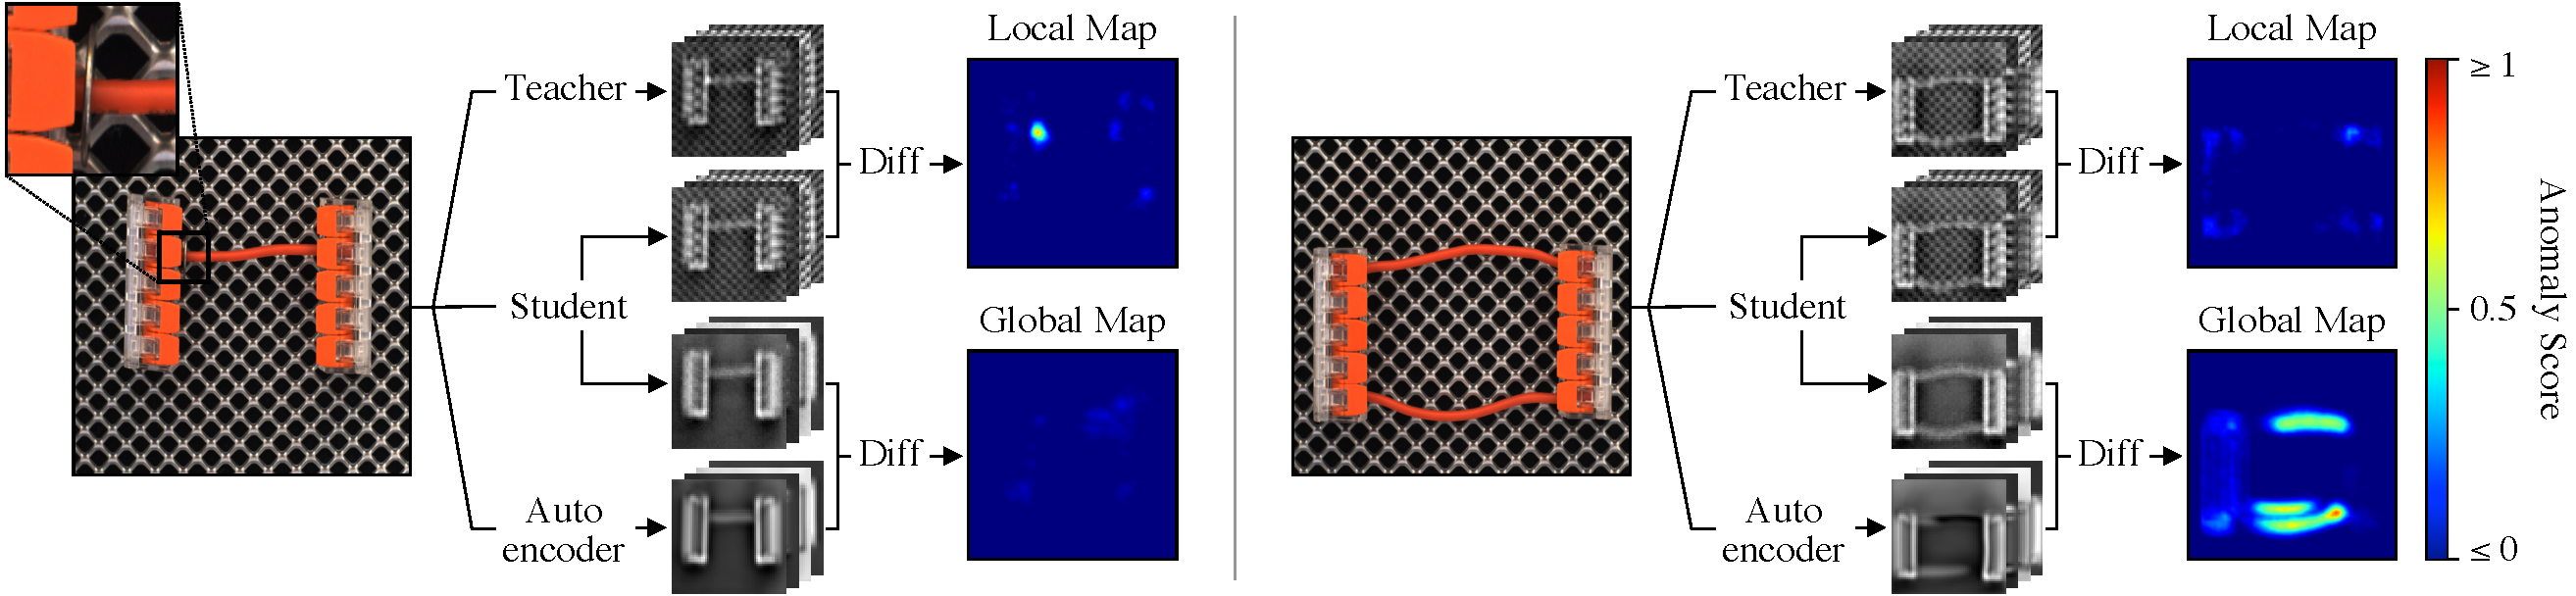
\includegraphics[width=1.1\linewidth]{Rohit_Master_Thesis/Images/efficientAD_pipeline.pdf}
    \caption{EfficientAD pipeline}
    \label{fig:EfficientAD pipeline}
\end{figure}

The student learns the systematic reconstruction errors of the autoencoder on normal images, but it doesn't learn the reconstruction errors for anomalies as they are not part of the training set. This makes the difference between the student's and the autoencoder's output suitable for computing the anomaly map, which is calculated as squared difference between the two outputs and then averaging across all channels. EfficientAD produces two anomaly maps, the one generated by autoencoder-student pair is called global anomaly map and the one generated by \gls{s-t} pair is called local anomaly map as seen in the figure \ref{fig:EfficientAD pipeline}. Then these two maps are normalized to similar scale and then averaged to generate the combined anomaly map, and its maximum value is used as image-level anomaly score \cite{batzner2024efficientadaccuratevisualanomaly}.

\paragraph*{Performance :}

EfficientAD achieves an impressive image-level \gls{auroc} score of $99.8\%$ on MVTec AD dataset\cite{8954181} with early stopping enabled. For the overall anomaly detection performance, EfficientAD achieves very strong image-level detection and pixel-level localization performance with a highest score of $98.1$ for VisA\cite{zou2022spotthedifferenceselfsupervisedpretraininganomaly} dataset. The computational cost of EfficientAD was measured using the metrics latency and throughput, with the EfficientAD showing latency of $2.2ms$ and throughput of 614 $img/s$ \cite{batzner2024efficientadaccuratevisualanomaly}.

\subsubsection{FastFlow}
\label{subsec:fastflow}

Most existing representation-based moethods uses a deep convolutional neural network to extract normal image features and are then characterized this distribution through non-parametric distribution estimation methods. But these methods fails to map features effectively to a tractable base distribution and ignore the relationship between the local and global features which are essential for anomaly detection. Therefore, FastFlow is proposed to mitigate these problems. FastFlow is an unsupervised anomaly detection and localization model which is built with 2D normalization flows as its probability distribution estimator. Experimental findings shows that FastFlow outperforms previous state-of-the-art methods in terms of both accuracy and inference efficiency. It achieves 99.4\% AUC in anomaly detection \cite{yu2021fastflowunsupervisedanomalydetection}.

\paragraph*{Core Concept :}

Earlier unsupervised approaches used non-parametric methods while recents ones started using normalization flow to model the distribution of features for normal images. However these one-dimensional normalization flow models  requires the flattening of the two-dimensional input feature into a one-dimensional vector to estimate the distribution which destroys the positional relationship of 2D image and limits the ability of flow model. These models also used sliding window approach to extract features from a large number image patches and detect anomalies for each patch, this led to high inference complexity. Therefore to address the above problems FastFlow which extends the normalizing flow to two-dimensional space by using fully connected neural networks as the subnet which can maintain the relative position of the space, and supports end-to-end inference of the whole image. This improves the anomaly detection performances and gives the detection and localization results at once for the whole image to improve inference efficiency \cite{yu2021fastflowunsupervisedanomalydetection}.

\begin{figure}[ht!]
    \centering
    \includegraphics[width=1.1\linewidth]{Rohit_Master_Thesis//Images/fastflow_pipeline.png}
    \caption{FastFlow pipeline\cite{yu2021fastflowunsupervisedanomalydetection}}
    \label{fig:fastflow pipeline}
\end{figure}

Figure \ref{fig:fastflow pipeline} shows the FastFlow pipeline, in which first the visual features are extracted using the feature extractor and then passed as an input to the FastFlow module for probability density estimation. During training FastFlow is trained using normal images to convert the normal distribution into a standard normal distribution in 2D manner. For inferencing, anomaly score is assigned  to each location on the two-dimensional feature based on its probability values \cite{yu2021fastflowunsupervisedanomalydetection}.

The FastFlow pipeline consists of two main components, they are:

1. Feature Extractor,

2. 2D Normalization Flow

\paragraph*{Feature Extractor :}

First step in the whole pipeline is to extract representative features from input image using either ResNet as explained in section \ref{subsec:ResNet} or \gls{vit}. In \glspl{vit} as feature extractor, features from only one layer are extracted because of its capability to capture the relationship between local patches and global features. In case of ResNet, features are taken from directly the last layer in the first three blocks, and then these features are inputted into three corresponding FastFlow model \cite{yu2021fastflowunsupervisedanomalydetection}. 

\paragraph*{2D Normalization Flow :}

The 2D flow function is used to project the image features into the hidden variable using a bijective invertible mapping. At the time of inference, the features of anomalous images should be out of distribution and therefore will have lower likelihoods than normal images. This likelihood can be use as the anomaly score. Secifically, the sum of 2D probabilities of each channel is done to obtain the final probability map, and then its upsampled to the input image resolution using bilinear interpolation. In order to convert the original normalization flow into a 2D format, an alternate $3\times3$ and $1\times1$ convolutional layers are used in the default subnet as shown in the figure\ref{fig:fastflow pipeline} to retain the spatial information in the flow model and the loIn the feature extraction stage, the features are extracted using \gls{dnn} as the backbone, such as ResNet[mention reference], which was pre-trained on ImageNet\cite{5206848} dataset \cite{10208786}., CIFAR-10\cite{krizhevsky2009learning}, BTAD\cite{Mishra_2021} datasets. For MVTec AD dataset, the FastFlow model was compared with many state-of-the-art models with two metrics image-level \gls{auc} and pixel-level \gls{auc}. FastFlow demonstrates exceptional performance in anomaly detection, achieving an 99.4 image-level \gls{auc}, and 98.5 pixel-level \gls{auc}, surpassing all the other models. In case of CIFAR-10 dataset, FastFlow achieves an \gls{auc} 66.7 which is the best performing model when compared with others. For the BTAD dataset, FastFlow again surpasses all the compared models and achieves a pixel-level \gls{auc} of 97.0 \cite{yu2021fastflowunsupervisedanomalydetection}.

\subsubsection{Deep Feature Kernel Density Estimation (DFKDE)}
\label{subsec:dfkde}

\gls{dfkde} is a fast one-class anomaly detection model. It consists of two stages:

1. Feature extraction stage,

2. Anomaly detection stage,

In the feature extraction stage, the features are extracted using \gls{dnn} as the backbone, such as ResNet[mention reference], which was pre-trained on ImageNet\cite{5206848} dataset \cite{10208786}. The penultimate layer which is the average pooling layer of the backbone is used to obtain a semantic feature vector of a fixed length of 2048 \cite{Anomalib2024}.

In the anomaly detection stage, once the features are extracted, then these features undergoes dimensionality reduction using \gls{pca}\cite{IBM2023} to get the first 16 principal components. \gls{pca} is among the simple and most straightforward ways of doing dimensionality reduction. Its a technique that reduces high-dimensional data into a lower-dimensional representation by using the dependencies between variables, without loosing too much information \cite{Shalizi2012}. After the features are reduced using \gls{pca}, then on these reduced features Gaussian \gls{kde} is applied. The main idea behind \gls{kde} is that the training datasets will follows some random distribution, and this distribution can be modelled by employing \gls{kde} \cite{10208786}.

During inference, if a lower probability density is observed below the threshold determined by the training dataset, this indicates the existence of an anomaly compared the data distribution learned from the training data \cite{10208786}. The \gls{dfkde} gives competitive results on MVTec AD\cite{8954181}, for the metric \gls{auroc} \gls{dfkde} gives highest of 96.5 score \cite{Anomalib2024}.

%see if I want to write about densenet architecture in the theory section.